 % !TEX root = report.tex
 % !TEX program = xelatex

本项目中全面运用了模块化的设计思想。在最初设计时(见图\ref{fig:design_architecture}),我们为项目设计了六个功能模块(键盘译码、渲染控制、UART发送与接收、VGA信号发生与处理)和一个调试模块。然而,终端本身功能的特点,即其事实上不对用户指令进行任何除译码外的处理,决定了其实这个系统中存在两条独立的信号通路,即:键盘输入→按键译码→UART发送,UART接收→指令处理→渲染→VGA输出。因此,在最终实现中(如图\ref{fig:final_architecture}),我们将项目分成了两个大模块,即键盘控制器\texttt{KeyboardController}与图形控制器\texttt{VideoController},二者分别处理上述的两条信号通路,完成各自的功能,互相独立。事实证明,这种解耦合的思想为我们的开发带来了很多的便利。

\begin{figure}[htbp]
\centerline{
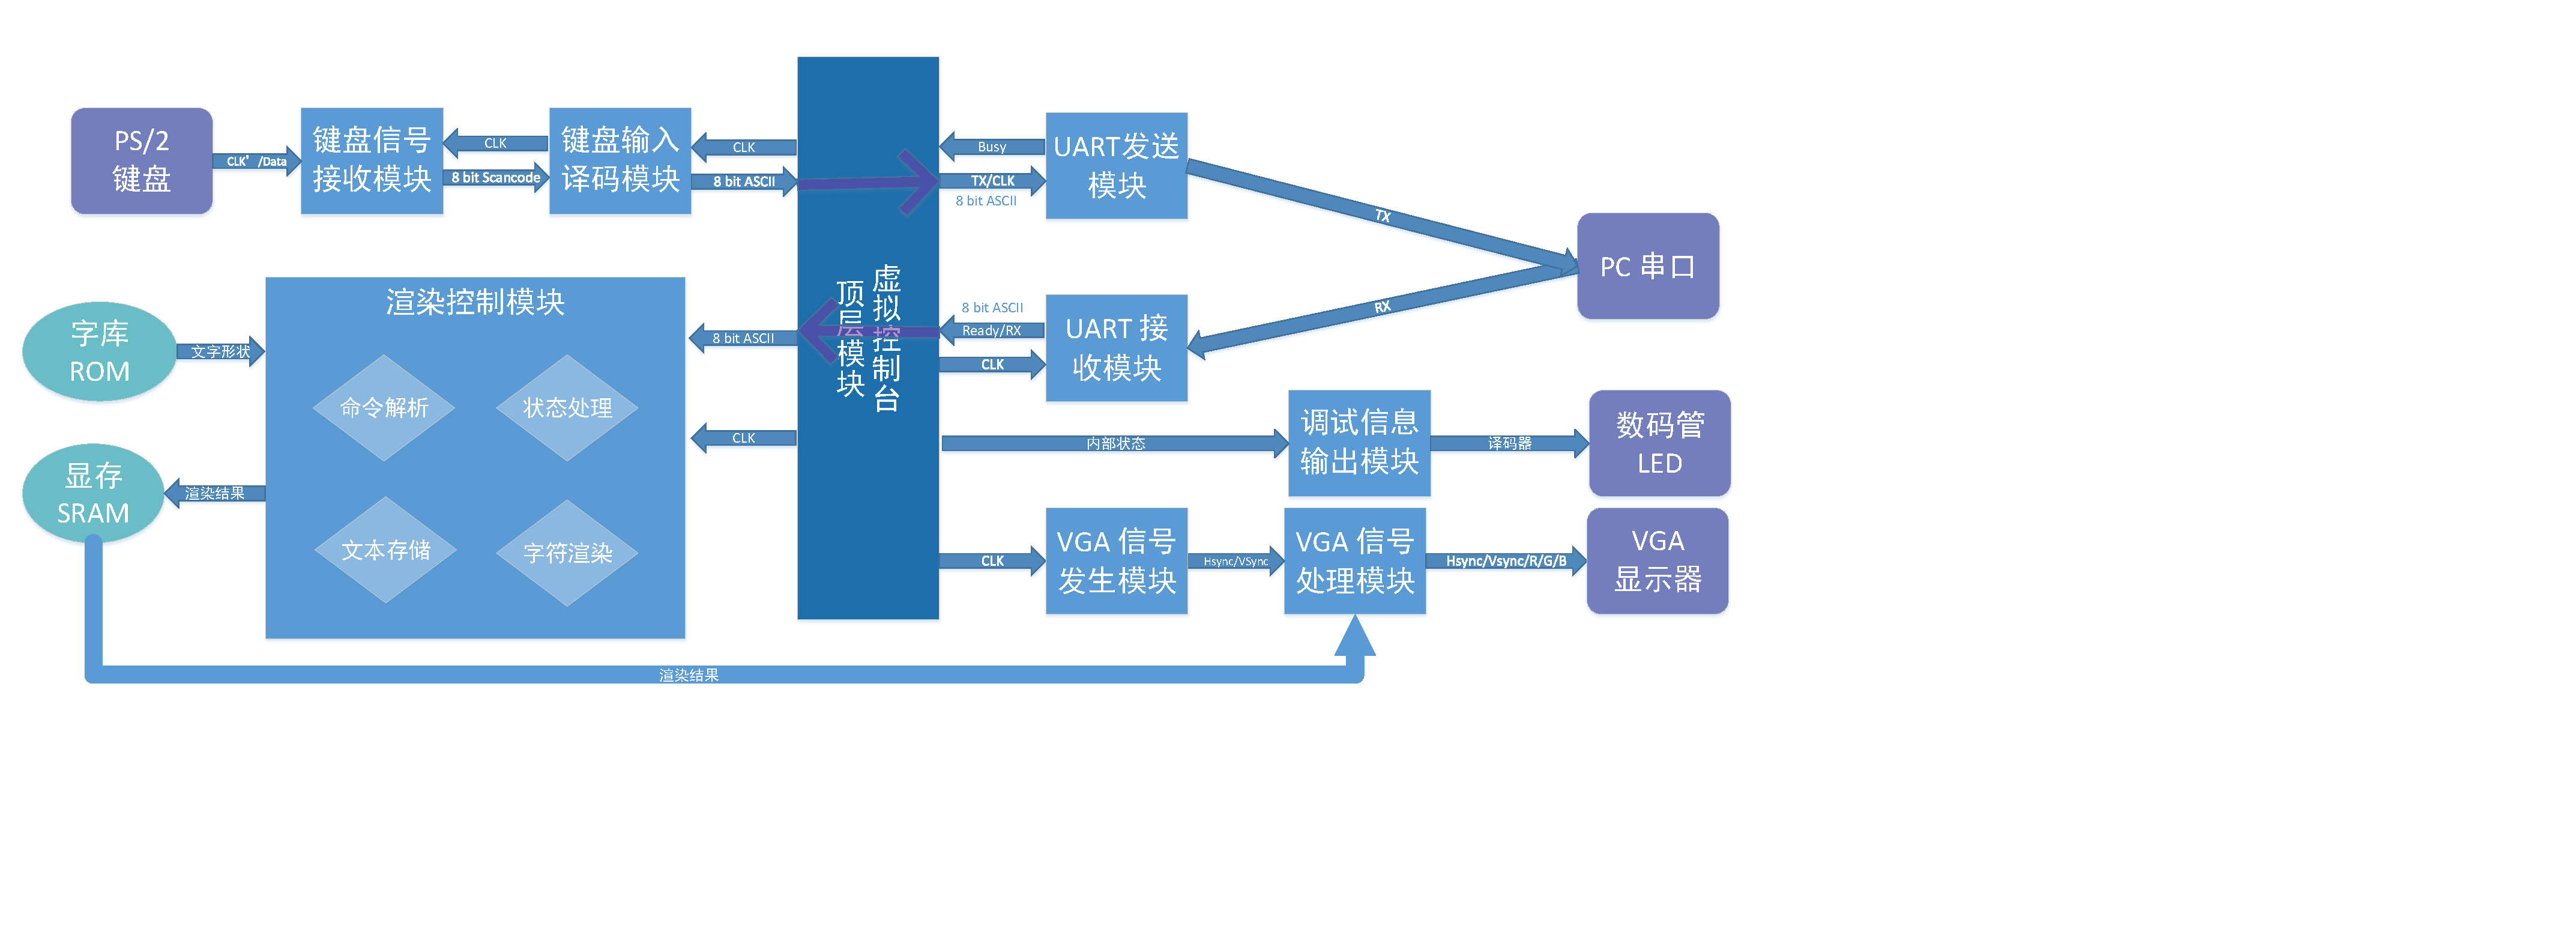
\includegraphics[width=0.95\paperwidth]{architecture_design_visio.pdf}
}
\label{fig:design_architecture}
\caption{项目设计架构}
\end{figure}

\begin{figure}[htbp]
\centerline{
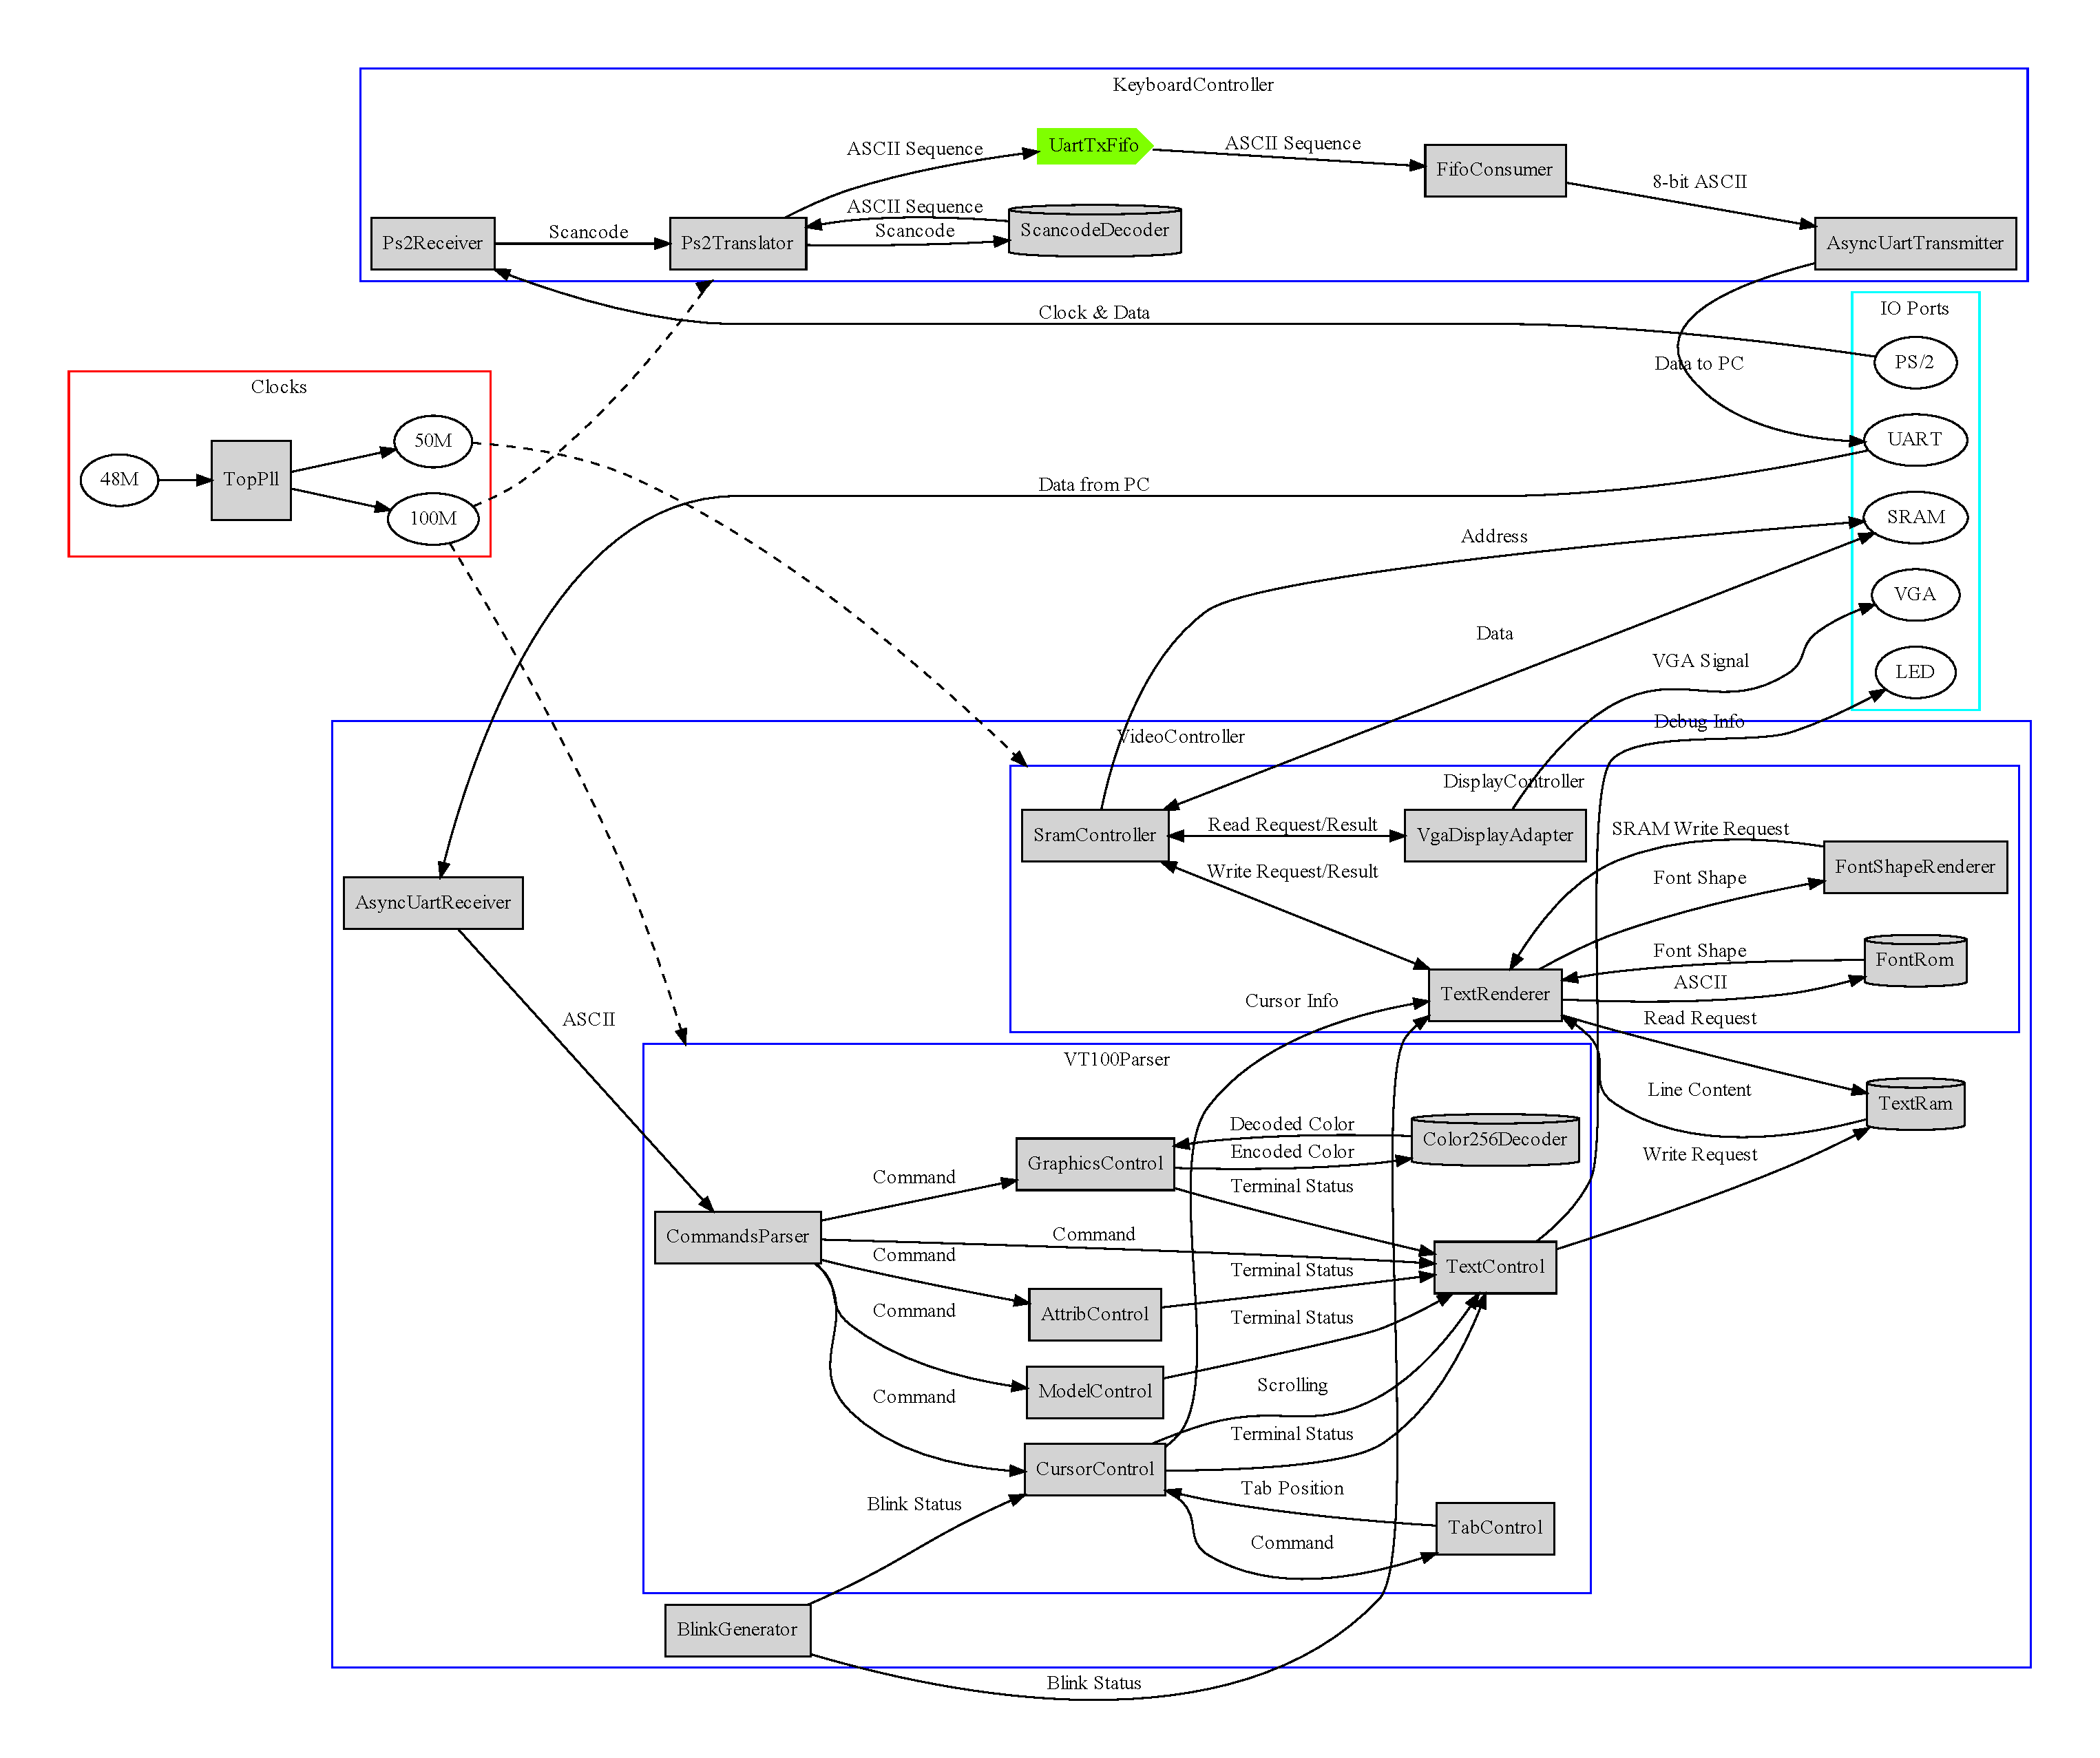
\includegraphics[width=\paperwidth]{architecture_final_dot.pdf}
}
\label{fig:final_architecture}
\caption{项目最终架构}
\end{figure}